\documentclass[12pt, a4paper]{article}

\usepackage{import}
\usepackage{standalone}

\usepackage[top=4cm, right=2cm, bottom=2.7cm, left=2cm]{geometry}

\usepackage{wrapfig}
\usepackage{tabulary}
\usepackage{float}
\usepackage{pifont}
\usepackage{background}
\usepackage{tikz}


\pagestyle{empty}
\setlength{\parindent}{0pt}

\begin{document}
	\begin{minipage}{\textwidth}
		\section{De Pijlen Veranderen \hfill\small Bron: Bebras}
			
			Deze opgave gebruikt 'vakjes' verbonden met 'pijlen'. Een opdracht, waarvoor we het teken := gebruiken, laat toe om een pijl te veranderen. De opdracht \textbf{A := B} bijvoorbeeld, verandert de pijl die vertrekt vanuit A. Nadat deze opdracht is uitgevoerd, zal de pijl die vertrekt vanuit A zodanig veranderd zijn dat ze nu aankomt op dezelfde plaats als de pijl die vertrekt vanuit B.
	
			\begin{figure}[H]
				\centering
				\large
				Voor \hspace{9cm} Na
				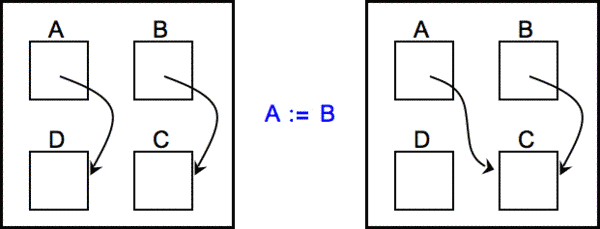
\includegraphics[width=\linewidth]{image1} 
			\end{figure}
	
			We willen nu de transformatie uitvoeren die hieronder is afgebeeld met behulp van een reeks van dergelijke opdrachten die de ene na de andere moeten worden uitgevoerd.
		
			\begin{minipage}{0.45\linewidth}
				\begin{figure}[H]
					\centering
					\large
					Voor
					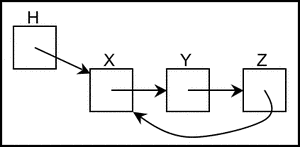
\includegraphics[width=\linewidth]{image2} 
				\end{figure}
			\end{minipage} \hfill
			\begin{minipage}{0.45\linewidth}
				\begin{figure}[H]
					\centering
					\large
					Na
					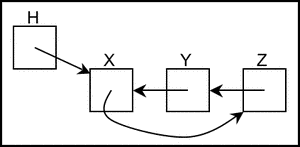
\includegraphics[width=\linewidth]{image3} 
				\end{figure}
			\end{minipage} \\

		
			Welke is de reeks opdrachten die hiervoor kan gebruikt worden?
		
			\begin{table}[H]
				\centering
				\begin{tabular}{|c|c|}
					\hline
					\textbf{A} & eerst \textbf{X := Z}, dan \textbf{Z := X}, dan \textbf{Y := H} \\
					\textbf{B} & eerst \textbf{X := Y}, dan \textbf{Y := Z}, dan \textbf{Z := X} \\ 
					\textbf{C} & eerst \textbf{Z := X}, dan \textbf{X := Y}, dan \textbf{Y := H} \\ 
					\textbf{D} & eerst \textbf{Z := Y}, dan \textbf{X := Z}, dan \textbf{Y := H} \\
					\hline 
				\end{tabular}
			\end{table}
	\end{minipage} \\ \\
	
\end{document}	